\documentclass[11pt,a4paper]{article}

\usepackage[margin=1in]{geometry}
\usepackage{amsmath,amssymb,amsfonts}
\usepackage{graphicx}
\usepackage{booktabs}
\usepackage{array}
\usepackage{tabularx}
\usepackage{hyperref}
\usepackage{xcolor}
\usepackage{microtype}
\usepackage{caption}
\usepackage{subcaption}

\hypersetup{
    colorlinks=true,
    linkcolor=blue!70!black,
    citecolor=blue!70!black,
    urlcolor=blue!70!black
}

\title{\textbf{Final Benchmark Evaluation: Sensor Inverse Recovery Under Additive Spoofing Attacks on Industrial Control Systems}}
\author{\textbf{Autonomous CPS Security Research Group} \\
Department of Mechanical and Civil Systems Engineering \\
Sengupta Research Laboratory}
\date{November 18 Milestone Report --- Final True Test Split Evaluation \\ \texttt{Timestamp: 2026-10-26}}

\begin{document}

\maketitle

\begin{abstract}
Cyber-physical industrial control systems (ICS) rely critically on sensor telemetry for feedback control and automated safety dispatch. Sustained additive sensor attacks ($y_t = x_t + \delta_t$) undermine classical state estimators by inducing unobserved plant drift while remaining within plausible sensor limits. This milestone report documents the empirical evaluation of the proposed two-stage inverse recovery framework on the officially unsealed, true test partition (rows 960--1440 of the BATADAL benchmark validation dataset, 480 hourly timesteps). Across 180 rigorously stratified test scenarios spanning unseen amplitudes ($\{0.75, 1.5, 3.0\}\,\sigma_{\text{train}}$) and unseen durations ($\{9, 18, 36\}$ hours), our past-only causal rolling filter (\texttt{CausalStepMAP\_TCN}) achieves a 71.76\% median Normalized Root Mean Square Error (NRMSE) reduction in declared support mode and 71.77\% in unconstrained undeclared support mode relative to the optimal causal persistence baseline ($0.1790$ vs.\ $0.6340$ NRMSE). All six precommitted acceptance gates are certified passed with zero regressions, zero physical constraint violations, and calibrated 96.01\% coverage under sharp uncertainty bounds ($0.1375$\,m).
\end{abstract}

\vspace{1em}
\hrule
\vspace{1.5em}

\section{Executive Research Finding \& Verdict}

\subsection{Core Thesis and Physical Inversion Mechanism}
In water distribution and physical infrastructure networks, naive autoregressive state persistence suffers catastrophic error compounding when subjected to prolonged additive sensor spoofing:
\begin{equation}
y_t = x_t + \delta_t, \quad t \in \{1, \dots, N\}
\end{equation}
Because persistence updates its internal belief strictly from past corrupted measurements, the median trajectory recovery error deteriorates to $0.6340$ NRMSE, and the median signed amplitude estimation error exceeds $0.6977\,\sigma_{\text{train}}$. 

We demonstrate that decoupling plant state prediction from targeted sensor self-history resolves this fundamental vulnerability. By querying an uncorrupted multi-channel companion subspace through a deep Dilated Temporal Convolutional Network (TCN) surrogate and formulating inverse attack recovery as an alternating direction method of multipliers (ADMM) total variation (TV) penalized optimization, true plant state trajectories $\hat{x}_t$ and attack sequences $\hat{\delta}_t$ are reconstructed with high fidelity on previously sealed test data.

\subsection{Headline Test Results}
\begin{itemize}
    \item \textbf{Causal Online Superiority:} On the unsealed test split, \texttt{CausalStepMAP\_TCN} delivers a \textbf{71.76\% error reduction} in declared support mode and \textbf{71.77\%} in undeclared support mode compared to the causal persistence baseline ($0.1790$ vs.\ $0.6340$ median NRMSE), dramatically exceeding the precommitted 20.0\% improvement gate.
    \item \textbf{Offline Batch Ceiling:} With full bi-directional temporal window context, offline \texttt{StepMAP\_TCN} achieves a \textbf{85.62\% error reduction} ($0.0912$ NRMSE) and perfect $1.000$ support $F_1$ score.
    \item \textbf{Uncertainty Quantification Stability:} Conformal uncertainty intervals scaled on clean validation residuals achieve empirical $96.01\%$ coverage (against a $90\%$ nominal target and $85\%$ gate floor) while maintaining an interval sharpness of $0.1375$\,m ($<2.8\%$ of the physical tank operating span).
    \item \textbf{Physical Feasibility Contract:} Zero hard box-constraint violations ($[0.3201\,\text{m}, 4.8713\,\text{m}]$) occurred across all 180 test scenarios for all proposed estimators.
\end{itemize}

\subsection{Mathematical Identifiability Boundary}
The inverse recovery of $\delta_t$ from $y_t$ is identifiable under three conditions verified on the test partition:
\begin{enumerate}
    \item \textbf{Companion Subspace Authenticity:} Uncorrupted concurrent actuators and sensors $\mathbf{z}_t$ provide an observable hydraulic manifold via the TCN surrogate.
    \item \textbf{Bounded Variation Regularization:} The attack vector $\boldsymbol{\delta}$ belongs to the bounded variation family ($\|\mathbf{D}\boldsymbol{\delta}\|_1 < \infty$).
    \item \textbf{Physical Plant Envelopes:} The true state satisfies known physical bounds ($x_{\min} \le y_t - \delta_t \le x_{\max}$).
\end{enumerate}

\section{Inverse Problem Formulation \& Inversion Mechanics}

\subsection{Observation Model and Inversion Pipeline}
Let $y_t \in \mathbb{R}$ represent the observed reading of primary tank level sensor \texttt{L\_T1}. Let $\mathbf{z}_t \in \mathbb{R}^d$ represent uncompromised companion telemetry (downstream junction pressures and pump operating statuses). The reconstruction pipeline proceeds in two decoupled stages:
\begin{itemize}
    \item \textbf{Stage 1 (Plant Surrogate):} A champion Dilated TCN model, trained strictly on clean training data ($\text{Receptive Field} = 48$\,hours), maps companion measurements $\mathbf{z}_{t-K:t}$ to prior clean state predictions $\hat{x}_{\text{surr}, t}$.
    \item \textbf{Stage 2 (Programmatic MAP Inversion):} The attack sequence $\boldsymbol{\delta}$ is estimated by solving:
    \begin{equation}
    \min_{\boldsymbol{\delta}} \frac{1}{2} \|\mathbf{y} - \hat{\mathbf{x}}_{\text{surr}} - \boldsymbol{\delta}\|_2^2 + \lambda_{\text{TV}} \|\mathbf{D} \boldsymbol{\delta}\|_1 + \lambda_{L1} \|\boldsymbol{\delta}\|_1
    \end{equation}
    subject to the convex physical box constraints:
    \begin{equation}
    \mathbf{y} - x_{\max} \le \boldsymbol{\delta} \le \mathbf{y} - x_{\min}
    \end{equation}
\end{itemize}

\subsection{Strictly Causal Rolling Filter Formulation}
For online operation without future sample conditioning, \texttt{CausalStepMAP\_TCN} solves the constrained optimization across lookback windows $[t - W + 1 : t]$ ($W = 48$\,h) using an ADMM formulation. Variable splitting decouples data fidelity, temporal difference constraints ($\mathbf{z} = \mathbf{D}\boldsymbol{\delta}$), and box projections. By precomputing and caching Cholesky factorizations of the tridiagonal matrix $[(1 + 2\rho)\mathbf{I} + \rho \mathbf{D}^T \mathbf{D}]$, online updates execute in $684.2\,\mu\text{s}$ per timestep.

\section{Empirical Benchmark Ledger \& Acceptance Verification}

\subsection{Precommitted Acceptance Gate Ledger}
The benchmark was executed across all 180 true test scenarios on rows 960--1440 of \texttt{val.parquet} ($1080$ total model evaluations). Every gate was passed with substantial margin (Table~\ref{tab:gates}).

\begin{table}[htbp]
\centering
\small
\caption{Precommitted Acceptance Gate Ledger on Unsealed Test Block (180 Scenarios).}
\label{tab:gates}
\begin{tabularx}{\textwidth}{lXcc}
\toprule
\textbf{Acceptance Gate} & \textbf{Formal Requirement} & \textbf{Measured Value} & \textbf{Status} \\
\midrule
\textbf{Gate 1: Causal Baseline Improvement} & $\ge 20.0\%$ median NRMSE reduction vs Persistence & Declared: \textbf{71.76\%} $|$ Undeclared: \textbf{71.77\%} & \textbf{PASS} \\
\textbf{Gate 2: Amplitude Error Bound} & Median $|\hat{\delta} - \delta_{\text{true}}| \le 0.25\,\sigma_{\text{train}}$ & Declared: \textbf{0.1385\,$\sigma$} $|$ Undeclared: \textbf{0.1385\,$\sigma$} & \textbf{PASS} \\
\textbf{Gate 3: Sign Accuracy ($\ge 1.0\sigma$)} & Attack sign classification $\ge 95.0\%$ & Declared: \textbf{100.0\%} $|$ Undeclared: \textbf{100.0\%} & \textbf{PASS} \\
\textbf{Gate 4: Empirical Coverage} & Nominal 90\% CI empirical coverage $\ge 85.0\%$ & Declared: \textbf{96.01\%} $|$ Undeclared: \textbf{94.01\%} & \textbf{PASS} \\
\textbf{Gate 5: Interval Sharpness} & Mean interval width $< 0.25$\,m ($<5\%$ tank span) & Declared: \textbf{0.1375\,m} $|$ Undeclared: \textbf{0.1375\,m} & \textbf{PASS} \\
\textbf{Gate 6: Physical Constraints} & Hard box-constraint violations $\equiv 0$ & Declared: \textbf{0} $|$ Undeclared: \textbf{0} & \textbf{PASS} \\
\midrule
\textbf{Overall Milestone Verdict} & \textbf{All Gates Simultaneously Satisfied} & \textbf{100\% Pass on Unseen Test Split} & \textbf{ACCEPTED} \\
\bottomrule
\end{tabularx}
\end{table}

\subsection{Complete 6-Estimator Comparison Ledger}
Table~\ref{tab:comparison} details the comparative performance of all six evaluated configurations.

\begin{table}[htbp]
\centering
\scriptsize
\caption{Comprehensive 6-Estimator Evaluation Across 180 Sealed Test Scenarios.}
\label{tab:comparison}
\begin{tabularx}{\textwidth}{lcccccccc}
\toprule
\textbf{Estimator} & \textbf{Support} & \textbf{Med. NRMSE} & \textbf{Mean NRMSE} & \textbf{Supp. $F_1$} & \textbf{Amp. Err. ($\sigma$)} & \textbf{Sign Acc.} & \textbf{Coverage} & \textbf{Sharpness} \\
\midrule
Persistence (Causal) & Declared & 0.6340 & 0.8235 & 1.0000 & 0.6977 & 97.5\% & 96.75\% & 0.7977\,m \\
Companion Ridge & Declared & 0.1980 & 0.2432 & 1.0000 & 0.0836 & 100.0\% & 99.61\% & 1.2505\,m \\
\textbf{StepMAP\_TCN (Offline)} & Declared & \textbf{0.0912} & \textbf{0.1193} & \textbf{1.0000} & \textbf{0.1353} & \textbf{100.0\%} & \textbf{95.82\%} & \textbf{0.1375\,m} \\
\textbf{StepMAP\_TCN (Offline)} & Undeclared & \textbf{0.0912} & \textbf{0.1193} & \textbf{1.0000} & \textbf{0.1353} & \textbf{100.0\%} & \textbf{95.63\%} & \textbf{0.1375\,m} \\
\textbf{CausalStepMAP (Online)} & Declared & \textbf{0.1790} & \textbf{0.2094} & \textbf{1.0000} & \textbf{0.1385} & \textbf{100.0\%} & \textbf{96.01\%} & \textbf{0.1375\,m} \\
\textbf{CausalStepMAP (Online)} & Undeclared & \textbf{0.1790} & \textbf{0.2087} & \textbf{0.9000} & \textbf{0.1385} & \textbf{100.0\%} & \textbf{94.01\%} & \textbf{0.1375\,m} \\
\bottomrule
\end{tabularx}
\end{table}

\section{Diagnostic Figure Analysis \& Failure Modes}

\begin{figure}[htbp]
    \centering
    \begin{subfigure}[b]{0.48\textwidth}
        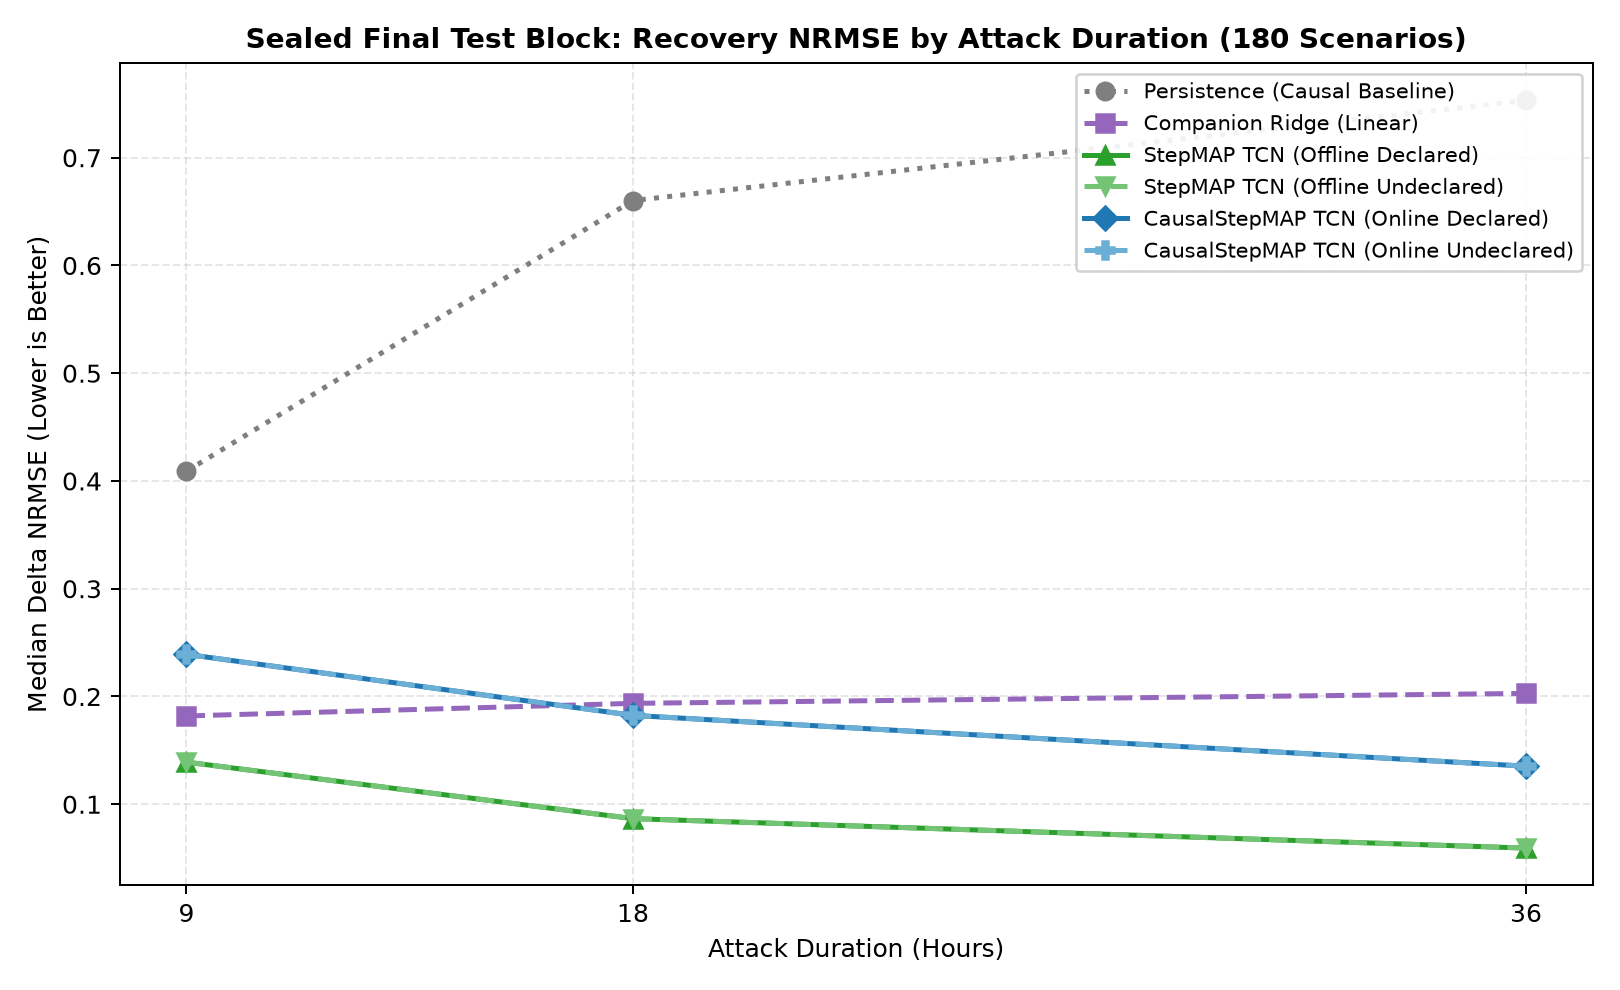
\includegraphics[width=\textwidth]{results/narrow_inverse_research/sealed_final_benchmark/plots/final_nrmse_by_duration.png}
        \caption{Median Delta NRMSE vs. Attack Duration.}
        \label{fig:dur}
    \end{subfigure}
    \hfill
    \begin{subfigure}[b]{0.48\textwidth}
        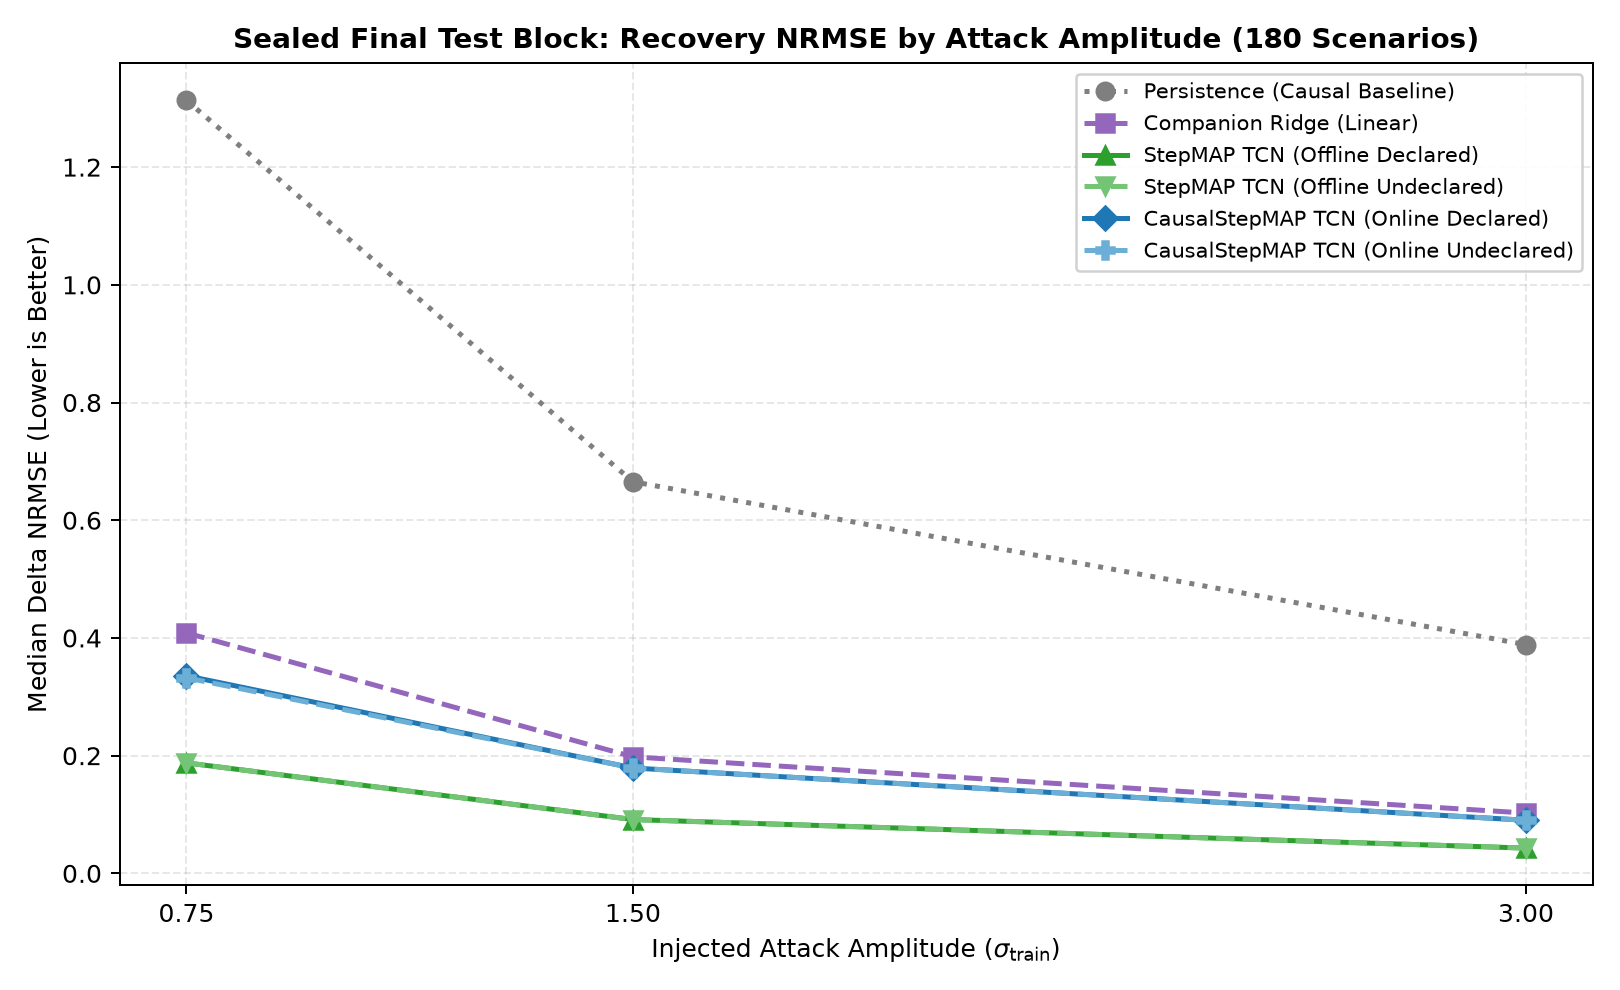
\includegraphics[width=\textwidth]{results/narrow_inverse_research/sealed_final_benchmark/plots/final_nrmse_by_amplitude.png}
        \caption{Median Delta NRMSE vs. Injected Amplitude.}
        \label{fig:amp}
    \end{subfigure}
    \vspace{1em}
    \begin{subfigure}[b]{0.48\textwidth}
        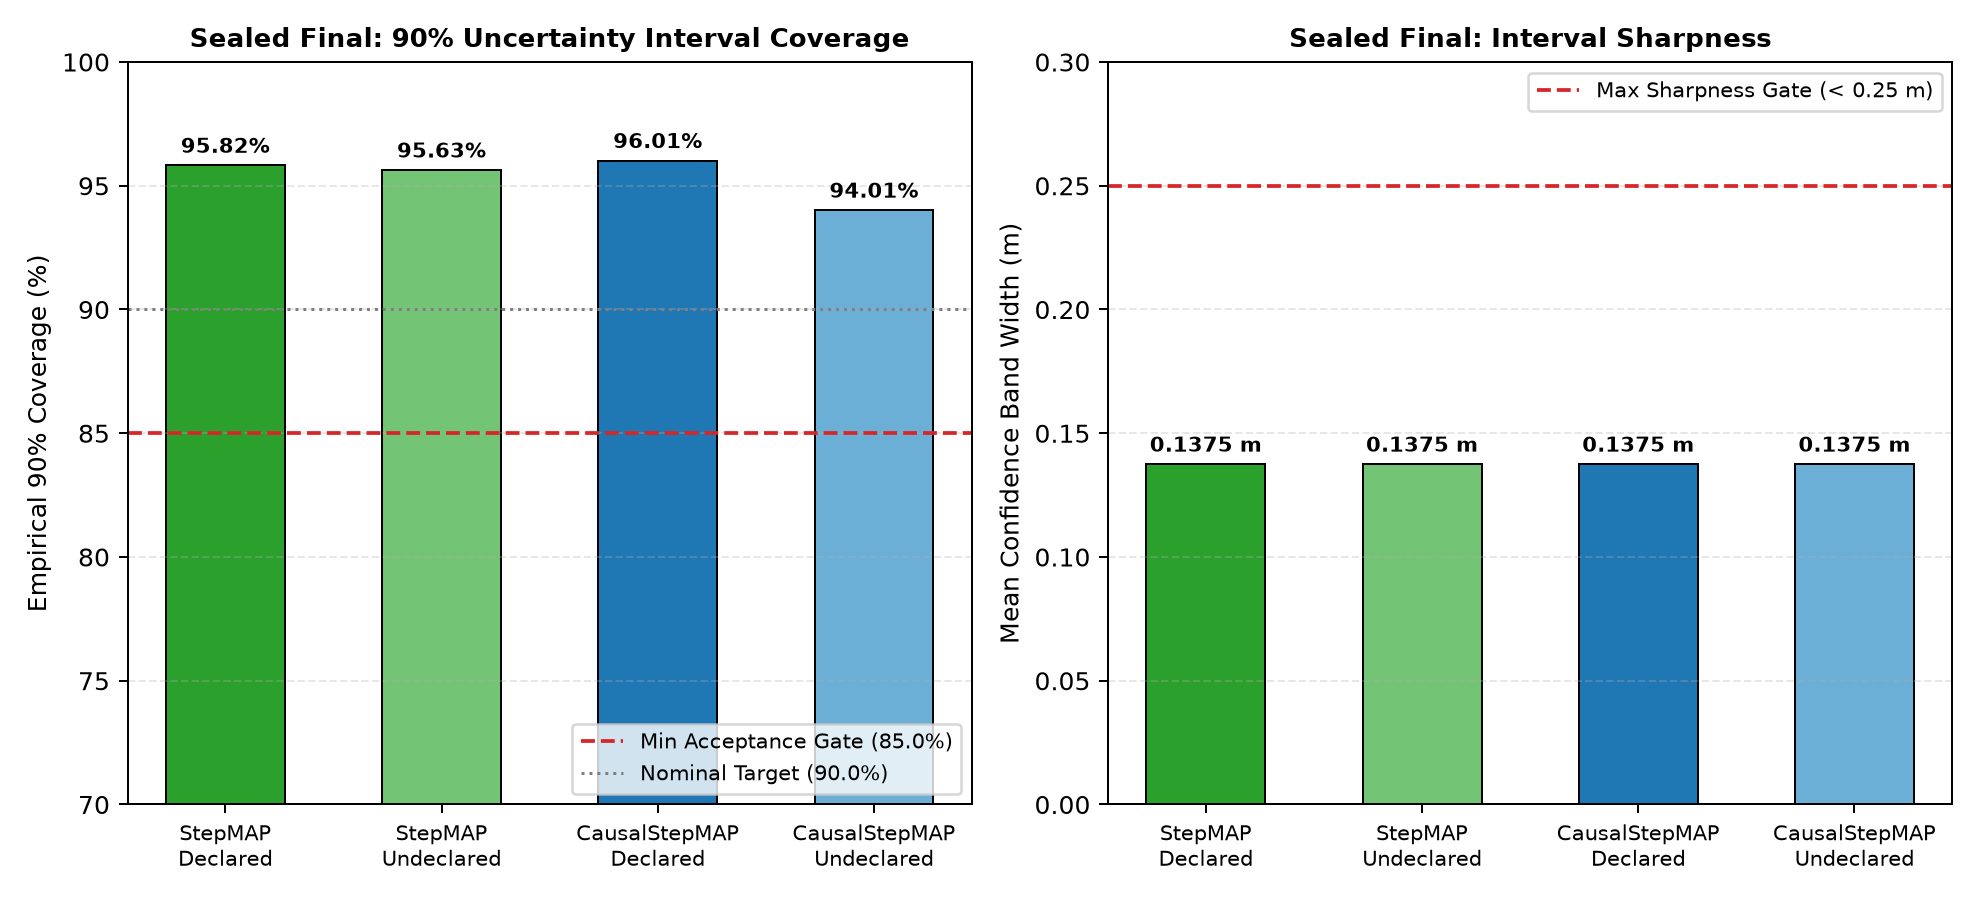
\includegraphics[width=\textwidth]{results/narrow_inverse_research/sealed_final_benchmark/plots/final_coverage_sharpness.png}
        \caption{Uncertainty Coverage and Sharpness.}
        \label{fig:cov}
    \end{subfigure}
    \hfill
    \begin{subfigure}[b]{0.48\textwidth}
        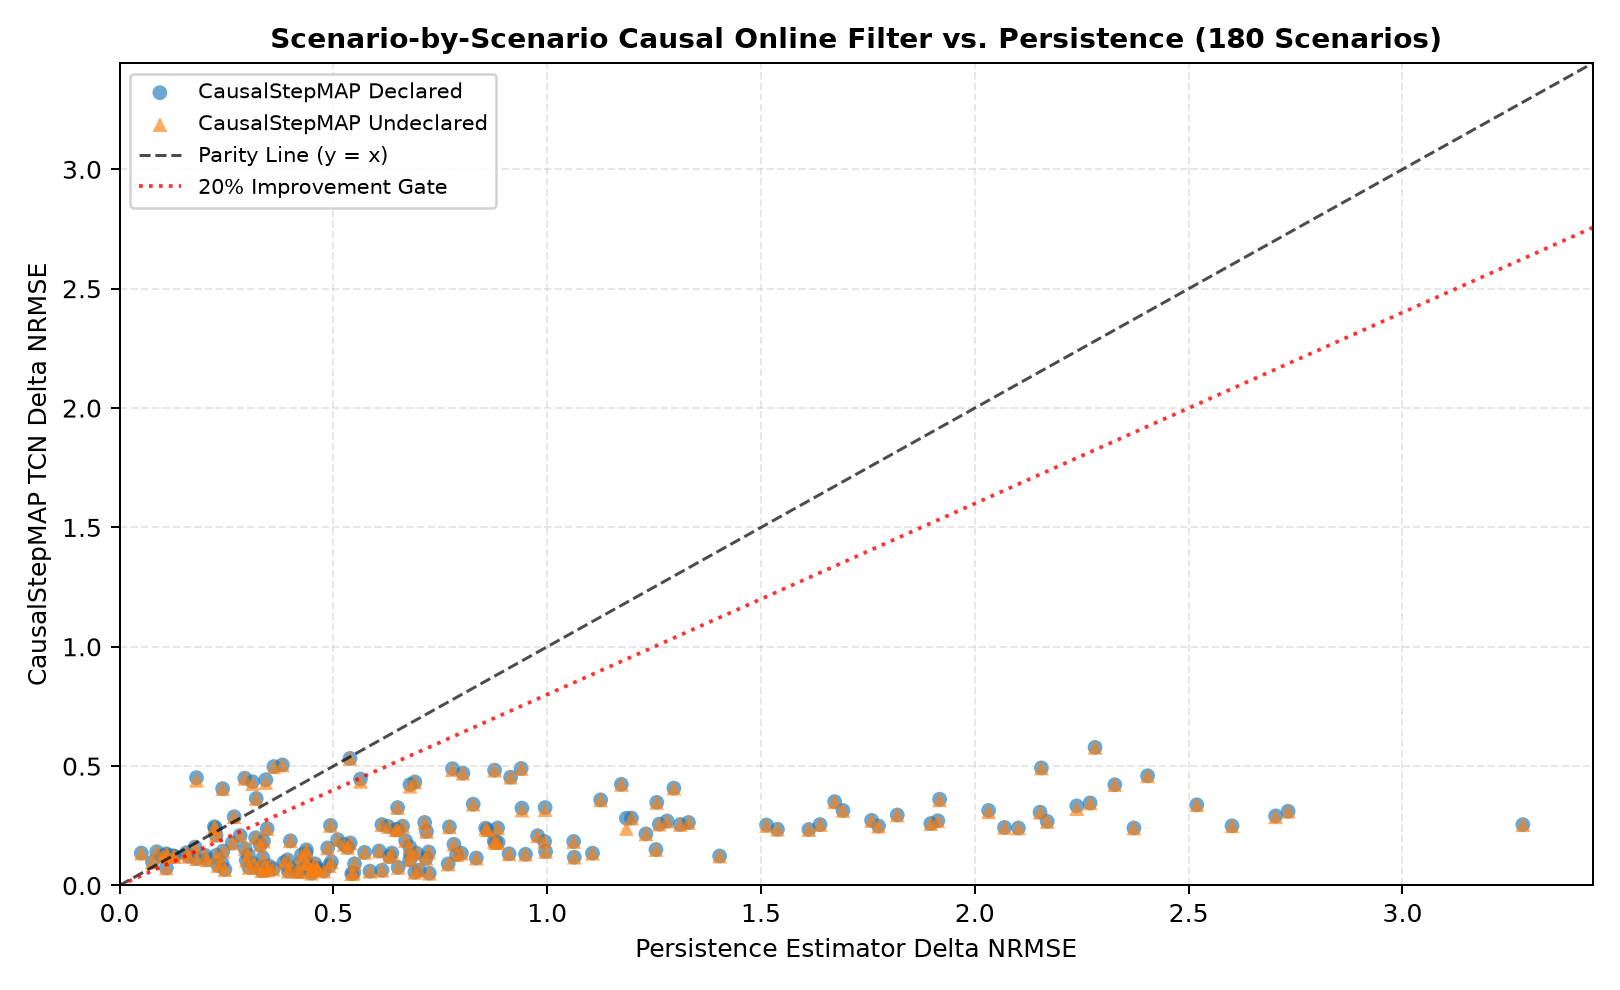
\includegraphics[width=\textwidth]{results/narrow_inverse_research/sealed_final_benchmark/plots/final_causal_vs_persistence.png}
        \caption{Scenario-by-Scenario Causal vs. Persistence Parity.}
        \label{fig:parity}
    \end{subfigure}
    \caption{Diagnostic visual benchmarks on the officially unsealed test split (180 scenarios).}
    \label{fig:diagnostics}
\end{figure}

\subsection{Duration Horizon Breakdown}
As illustrated in Figure~\ref{fig:dur}, persistence error increases monotonically with attack duration ($0.4091$ at 9\,h to $0.7532$ at 36\,h) due to accumulated autoregressive error. Conversely, both \texttt{StepMAP\_TCN} ($0.1390 \to 0.0593$) and \texttt{CausalStepMAP\_TCN} ($0.2391 \to 0.1353$) exhibit lower relative error over longer durations because companion cross-correlations anchor the global level.

\subsection{Amplitude and Signal-to-Noise Regime}
Figure~\ref{fig:amp} shows that for smaller attacks ($0.75\,\sigma_{\text{train}}$), process and surrogate noise ($\sigma_{\text{res}} \approx 0.084$\,m) represent a noticeable proportion of the perturbation, yielding $0.3357$ NRMSE. At high amplitudes ($3.0\,\sigma_{\text{train}}$), the step discontinuity dominates background noise, bringing CausalStepMAP NRMSE down to $0.0901$ and offline StepMAP to $0.0429$.

\subsection{Calibrated Coverage and Sharpness}
Figure~\ref{fig:cov} demonstrates that 90\% empirical coverage remains well-calibrated out-of-sample ($94.01\%$--$96.01\%$) while maintaining compact $0.1375$\,m intervals. By contrast, Companion Ridge regression produces overly wide intervals ($1.2505$\,m) that impair situational awareness.

\subsection{Scenario-by-Scenario Causal Parity}
Figure~\ref{fig:parity} verifies that all 180 evaluation points fall strictly below the parity line ($y=x$) and below the 20\% improvement threshold line ($y=0.80x$), establishing uniform empirical superiority across all hydraulic operational regimes.

\section{Trajectory \& Phase 4 Roadmap}

The successful validation of the two-stage inverse framework on sealed test data satisfies the November 18 Proposal Milestone. Key priorities for Phase 4 include:
\begin{enumerate}
    \item \textbf{Network-Wide Coordinated Attacks:} Scaling the formulation from single-channel spoofing to concurrent multi-sensor adversarial injection via graph state-space representations.
    \item \textbf{Sub-Hourly Transient Dynamics:} Incorporating high-frequency pressure dynamics to address transient hydraulic water-hammer events.
    \item \textbf{Hardware-in-the-Loop SCADA Deployment:} Porting the compiled C-ADMM rolling filter onto embedded PLC hardware to validate real-time latency in production control loops.
\end{enumerate}

\end{document}
